%% LyX 2.3.6.1 created this file.  For more info, see http://www.lyx.org/.
%% Do not edit unless you really know what you are doing.
\documentclass[english]{article}
\usepackage{lmodern}
\usepackage[T1]{fontenc}
\usepackage[latin9]{inputenc}
\usepackage{babel}
\usepackage{amsmath}
\usepackage{amsthm}
\usepackage{amssymb}
\usepackage{graphicx}
\usepackage[unicode=true,pdfusetitle,
 bookmarks=true,bookmarksnumbered=false,bookmarksopen=false,
 breaklinks=false,pdfborder={0 0 1},backref=false,colorlinks=false]
 {hyperref}

\makeatletter
%%%%%%%%%%%%%%%%%%%%%%%%%%%%%% Textclass specific LaTeX commands.
\numberwithin{equation}{section}
\numberwithin{figure}{section}
\theoremstyle{plain}
\newtheorem{thm}{\protect\theoremname}
\theoremstyle{plain}
\newtheorem{prop}[thm]{\protect\propositionname}

\makeatother

\providecommand{\propositionname}{Proposition}
\providecommand{\theoremname}{Theorem}

\begin{document}
\title{Analysis of a Target Cell Limited Model for Covid-19 Antibody Treatment }
\maketitle
\begin{abstract}
Mathematical models have become almost indispensable in characterizing the within-host viral dynamics of COVID-19. The information revealed by a model is valuable for understanding the pathogensis and developing antiviral drugs, in which drug effects are often incorporated as fold changes in certain parameter values. The target cell limited (TCL) model is arguably the most widely used model to study COVID-19 viral dynamics. In the context of incorporating COVID-19 antibody treatment in the TCL model, we discover a non-monotonic relationship between viral load reduction and the drug effect. This non-monotonic relationship is demonstrated by numerical simulations and confirmed with mathematical analysis in this paper. Our finding raises serious skepticism of the use of TCL model before this non-monotonic relationship can be verified with experimental or clinical investigations. Our analysis of other aspects of the TCL model appears to be more assuring. Our global stability analysis shows that the viral load always raise and then decline to zero through a period of an infection, which explains why the TCL model so effective in capturing the pattern of acute viral infection very well. In addition, our analysis supports and offers an explanation for applying the treatment before the viral load peaks, which is in agreement with other studies.      
\end{abstract}
\section{Introduction}
Coronavirus disease 2019 (COVID-19) has had a profound impact on the world, leading to numerous fatalities, widespread illness, and significant economic disruption. The disease is caused by the severe acute respiratory syndrome coronavirus 2 (SARS-CoV-2). The within-host viral dynamics of COVID-19 is the focus of numerous studies. A firm understanding of viral dynamics of SARS-CoV-2 infection and its association with disease progression is crucial for understanding the pathogenesis and developing treatment.  Real-time reverse transcription polymerase chain reaction (rRT-PCR) is a common testing method for COVID-19. This technique also offers quantitative measurement of viral load (VL). There are plenty of time series data of VL which offer valuable information of viral dynamics. In combination with data, mathematical models are frequently used to characterize viral dynamics and play an important role in many tasks to improve health, such as identify high risk groups, drug development and treatment planning.      

There are many sophisticated mathematical models of COVID-19 with-host viral dynamics, which take into account detailed mechanisms including adaptive immune response.  Nevertheless, the target cell limited (TLC) model and its variants, which was originally used for influenza \cite{baccam2006kinetics}, have been used in many studies to model Covid-19 within-host viral dynamic \cite{Wang_2020,Vaidya_2021,N_ant_2021} and to assist decision making in drug development and clinical treatment \cite{gonccalves2020timing}. This model focuses on the acute viral infection and is based on the assumption that the host cells, epithelial cells of the lung, are limited and do not regenerate within the time frame of interest. The model generally fits well to data of VL in samples such as nasopharyngeal swabs measured using rRT-PCR. 

Drug effects are usually modeled as a reduction or increase in the one or more parameters' values that is deemed to be appropriate considering the mechanism how the drug works \cite{Kim_2021}. Antibody drugs are believed to block the entry of the free virus into the host cell. Thus the drug effects are modeled by reduction of the parameter value that represent infection rate. However, some counter-intuitive results are found (internal communication) when examining the length of time for which the VL
remains the detectable level. It is urgent to gain a thorough understanding of the TCL model.

In Section \ref{sec:model-simulation}, we revisit the TCL model and conduct an comprehensive sensitivity analysis of the infection rate parameter and treatment time. Section \ref{sec:math-analysis} focuses on mathematical analysis, which confirms our findings from the numerical simulation conducted in Section \ref{sec:model-simulation}. Section \ref{sec:discussion} concludes the paper with a discussion of our results (more?).   


\section{Model description and simulation} \label{sec:model-simulation}
%\section{Sensitivity analysis of $\beta$ and treatment time}
\subsection{TCL model}
The TCL model \cite{baccam2006kinetics} we considered in our analysis take into account target cell density, infected cell density  and free virus density at time $t$ denoted respectively $T(t), I(t)$ and $V(t)$. Their dynamics are described by three ordinary differential equations as follows  
\begin{subequations}\label{eq:TCL-og}
\begin{eqnarray}
\frac{dT}{dt} & = & -\beta VT \\
\frac{dI}{dt} & = & \beta VT-\delta I \\
\frac{dV}{dt} & = & pI-cV,
\end{eqnarray}
\end{subequations}
where $\beta$ is the infection rate, $p$ is the production rate of free virus per infected cell, and $\delta$ and $c$ are the clearance rate for infected cells and free virus. There is a time-delayed version taking into account the eclipse phase of the infected cells:
\begin{subequations}\label{eq:TCL-delay}
\begin{eqnarray}
\frac{dT}{dt}      & = & -\beta VT\\
\frac{dI_{1}}{dt} & = & \beta VT-kI_{1}\\
\frac{dI_{2}}{dt} & = & kI_{1}-\delta I_{2}\\
\frac{dT}{dt}      & = & pI_{2}-cV,
\end{eqnarray}
\end{subequations}
where $I_1$ is the infected cells in the eclipse phase and $I_2$ is the infected cells that are capable producing free virus. $k$ is the parameter controls the length of the time delay. 

\subsection{Sensitivity analysis of drug effects and treatment time}
In this section, we examine the TLC model with the nominal parameter values reported by XX using numerical simulations. In the original study, this model was used to study an antibody drug against COVID-19. The original study decided to make the drug effect as a reduction in the infection rate $\beta$ but failed to estimate the efficacy concentration of the drug. Instead, it is claimed that at the given dose the drug effect is nearly saturated. This claim seems dubious and the saturated drug effect may be inevitable consequence due to the nature of the TCL model (likely a model artifact rather than faithful representation of the reality). 

Here, we consider VL falling below the level of quantification (LOQ) as the end point. We investigate the sojourn time VL above LOQ as the drug effect and treatment time are varied. By a comprehensive simulation-based sensitivity analysis, we plot the days of VL beyond LOQ as a function of the drug effect (a fraction of the nominal $\beta$ value) and treatment time (in days after infection) (left panel of Fig. \ref{fig:sojourn-time-slope}). The drug effect at 1 serves as the control (no reduction in $\beta$) to offer a baseline value of sourjon time. With the nominal parameter values, the model shows peaked VL around Day 6 after infection, which roughly coincides with the observed symptom onset of a patient. The interesting part is the non-monotonic relationship between the sourjon time and the drug effect for treatments applied between Day 2 and Day 6. It is surprising to find out that moderate reduction in $\beta$ leads to longer and plausibly unrealistic sourjon time (in some cases more than 60 days). Furthermore, there is a sharp decline in sourjon time as $\beta$ is further reduced and only extremely small $\beta$ reduces the sourjon time below the baseline. This is also illustrated in Fig. \ref{fig:logVL-days} where the log VL is plotted against days after infection. To fit the data and explain the reduction in VL due to the drug effect, very large reduction in $\beta$ is needed. So a dubious conclusion may be drawn that the drug effect saturated for all the given dose. On the right panel of Fig. \ref{fig:sojourn-time-slope}, the asymptotic reduction rate of VL is plotted and shows similar pattern. The analytically derived threshold {\eqref{eq:beta-critical}} for the drug effects for which the VL reducation rate starts decrease with stronger drug effects (smaller $\beta$) is overlay on the heat map showing its agreement with the numerical simulation (right panel of Fig. \ref{fig:sojourn-time-slope}).     

It appears that the drug has indiscernible effects on the sourjon time if the treatment is applied after Day 6 as seen from the homogeneous color or flat surface after Day 6 in Fig. \ref{fig:sojourn-time-slope}. This implies the importance of treating COVID-19 with antiviral drugs before the VL peaks. Similar findings have been reported in \cite{gonccalves2020timing}. In the Section \ref{sec:dynmaic-details}, our analysis of the model dynamics offers further support and explanation for this treatment timing preference.      
%It is included because the asymptotic reduction rate of VL estimated from simulation may be compared to the ones obtained from a analytical approach (to do). 

\begin{figure}
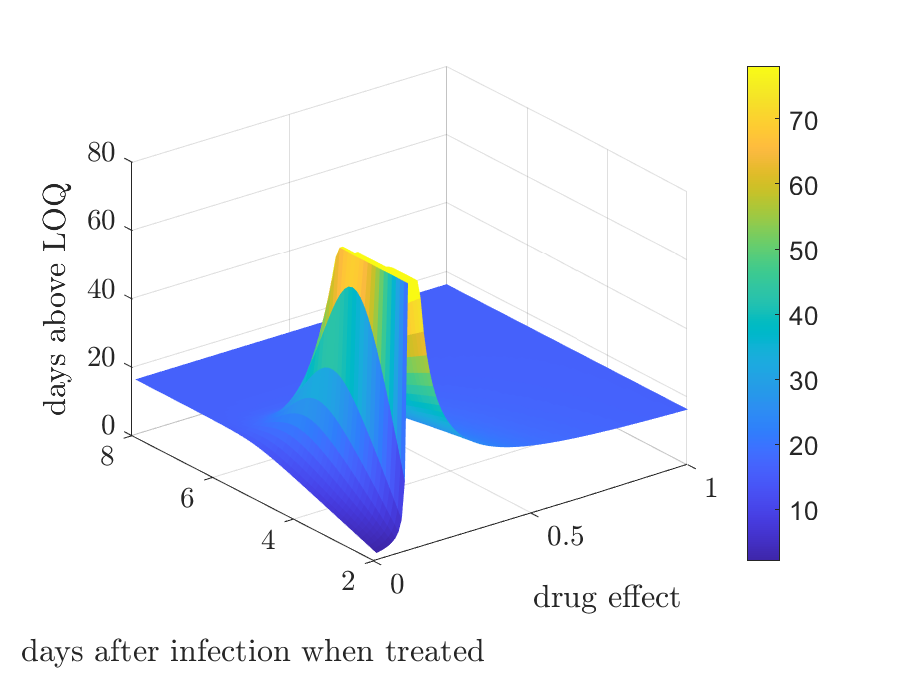
\includegraphics[width=0.48\linewidth]{figs/days_above_LOQ_vs_drug_days}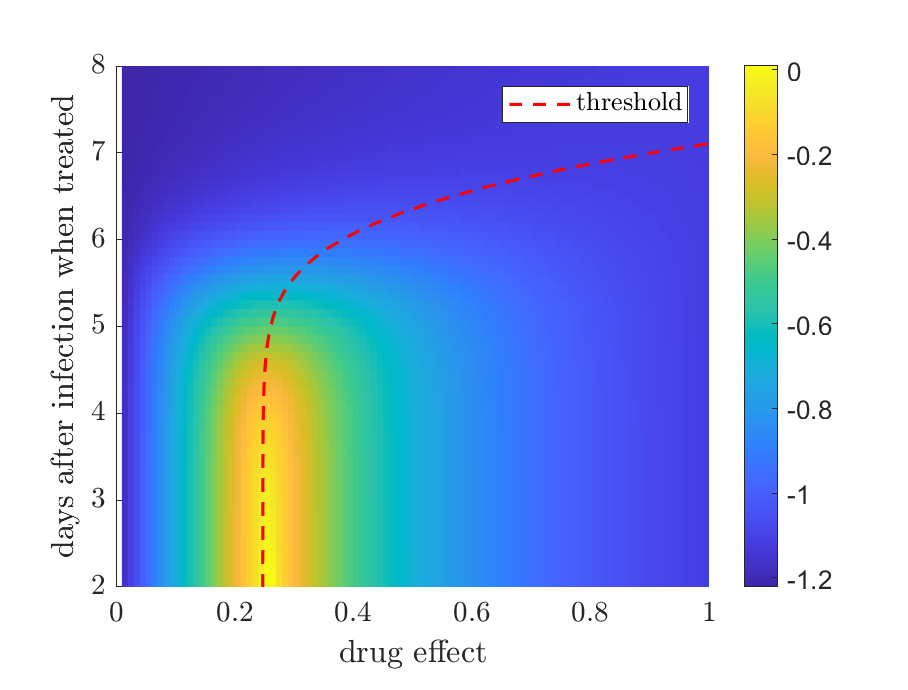
\includegraphics[width=0.48\linewidth]{figs/slope_vs_drug_days_threshold}\caption{Left: sojourn time of VL; right: asymptotic reduction rate of VL \label{fig:sojourn-time-slope}}
\end{figure}

\begin{figure}
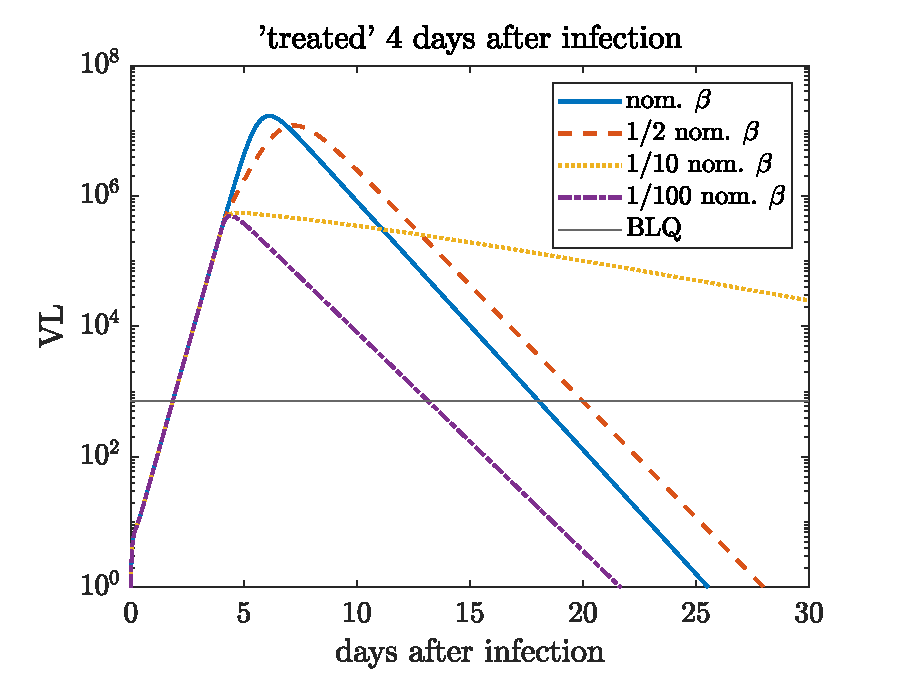
\includegraphics[width=0.48\linewidth]{figs/logVL_vs_time_day4tr_beta_100}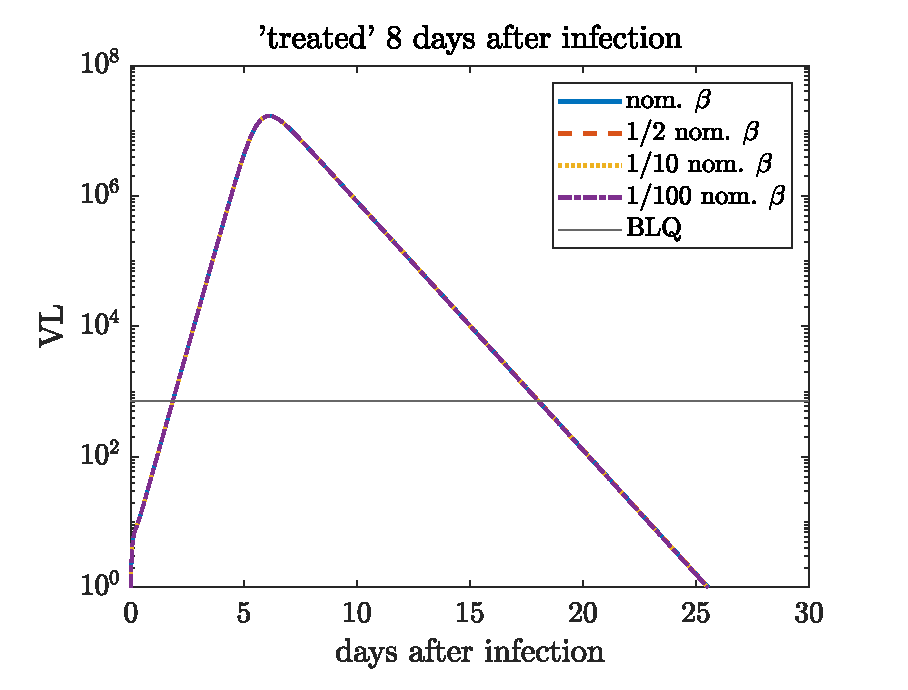
\includegraphics[width=0.48\linewidth]{figs/logVL_vs_time_day8tr_beta_100}\caption{logVL vs days after infection. Left: treated at Day 4; right: treated
at Day 8 \label{fig:logVL-days}}
\end{figure}


\section{Mathematical analysis} \label{sec:math-analysis}
We conduct mathematical analysis to confirm our findings from numerical simulations in the previous section.  Section \ref{sec:global-stability} involves standard analysis that assures that the TCL model is well behaved (solutions are bounded and non-negative) and suitable for describing an acute viral infection ($V(t)$ , representing the VL, raises at the beginning of an infection and eventually declines towards zero). In Section \ref{sec:dynmaic-details}, using an approximation enabled by separation of time scales, we derive a relationship between the VL reduction rate and $\beta$, as well as a few other results of interests from the perspective of modeling viral dynamics.      

\subsection{Global stability } \label{sec:global-stability}
We conduct our analysis of the TCL model without time delay \eqref{eq:TCL-og} and
note that many results obtained here can be easily generalize to the
time-delayed version \ref{eq:TCL-delay}. To facilitate analysis, we conduct nondimensionlization
of the system \eqref{eq:TCL-og} by introducing the dimensionless variables $\hat{t}=\frac{t}{t_{c}}$
, $\hat{T}=\frac{T}{T_{c}}$ , $\hat{I}=\frac{I}{I_{c}}$ and $\hat{V}=\frac{V}{V_{c}}$, where
the characteristic scales are $t_{c}=\delta t,V_{c}=\frac{1}{\beta t_{c}},T_{c}=I_{c}=\frac{\delta c}{\beta p}$. This gives the following dimensionless system
\begin{subequations} \label{eq:TCL-nondim}
\begin{eqnarray}
\frac{d\hat{T}}{d\hat{t}} & = & -\hat{T}\hat{V}\nonumber \\
\frac{d\hat{I}}{d\hat{t}} & = & \hat{T}\hat{V}-\hat{I}\nonumber \\
\frac{d\hat{V}}{d\hat{t}} & = & \frac{1}{\epsilon}(\hat{I}-\hat{V})\label{eq:cont-delay-2}
\end{eqnarray}
\end{subequations}
where $\epsilon=\delta/c$. We will drop the hats ($\hat{\,}$) for the dimensionless
variables for notional convenience. Since all variables are cell or
virus density, we focus on the non-negative orthant denoted by $\mathbb{R}_{+0}^{3}$,
which is not only biological relevant but also positive invariant,
i.e. any solution of \eqref{eq:TCL-nondim} that starts in $\mathbb{R}_{+0}^{3}$ stays in
the $\mathbb{R}_{+0}^{3}$. Boundedness of the solutions can be seen
by noting that $(T+I+\epsilon V)'=-V\le0$. So $T+I+\epsilon V\le T(0)+I(0)+\epsilon V(0)$.
We summarize the boundedness and negativeness of the solution as follows
\begin{prop}
(boundedness) Solutions of the system that starts in $\mathbb{R}_{+0}^{3}$
stays in $\mathbb{R}_{+0}^{3}$ and are bounded for all time.
\end{prop}

The equilibrium of the system \eqref{eq:TCL-nondim} is $(T^{*},0,0)$. Its Jacobian 
\[
\begin{bmatrix}0 & 0 & -T^{*}\\
0 & -1 & T^{*}\\
0 & \frac{1}{\epsilon} & -\frac{1}{\epsilon}
\end{bmatrix}
\]
 has characteristic polynomial $p(\lambda)=\lambda((\lambda+1)(\lambda+\frac{1}{\epsilon})-\frac{1}{\epsilon}T^{*})$.
It has positive eigenvalues if $T^{*}>1$ or in dimensional form
\begin{equation}
R_{0}\equiv\frac{\beta pT(0)}{c\delta}>1.\label{eq:R0}
\end{equation}
So the $(T^{*},0,0)$ with $T^{*}>1$ is unstable. That is, the infection
can occur. Here $R_{0}$ is often known as the reproduction number.
$T^{*}\le1$ there is a zero eigenvalue so that linear stability analysis
is inconclusive regarding to stability. Instead, we can show global
(Lyapunov) stability of $(T^{*},0,0)$ for $T^{*}\le1$ using a Lyapunov
function . We first show that 
\begin{prop}
For solutions of the system that starts in $\mathbb{R}_{+0}^{3}$,
$\{(T,I,V)\in\mathbb{R}_{+0}^{3}:T\le1\}$ is a global attractor.
\end{prop}
\begin{proof}
Since $T'\le0$. Thus the $\lim_{t\to\infty}T=\alpha$ exists. Suppose
$\{(T,I,V)\in\mathbb{R}_{+0}^{3}:T\le1\}$ is not global attractor.
Then we must have $\alpha>1$. By Babalat lemma, $\lim_{t\to\infty}T'=0$,
which implies that $\lim_{t\to\infty}V=0$ and $\lim_{t\to\infty}I=0$.
However this contradict with the fact $(\alpha,0,0)$ is unstable. 
\end{proof}
In $\{(T,I,V)\in\mathbb{R}_{+0}^{3}:T\le1\}$, the global stability follows. So we have 
\begin{thm}
(Global stability) The equilibrium $(T^{*},0,0)$ with $T^{*}\le1$
is Lyapunov stable.
\end{thm}
\begin{proof}
Consider the following Lyapunov function
\[
V=T-T^{*}\ln T+\frac{1}{2}I^{2}+\frac{1}{2}V^{2}
\]
 in $\{(T,I,V)\in\mathbb{R}_{+0}^{3}:T<1\}$. Then its derivative
with respect to time is given by
\begin{eqnarray*}
\frac{dV}{dt} & = & -TV-T^{*}V+II'+VV'\\
 & \le & I(TV-I)+V\frac{1}{\epsilon}(I-V)\\
 & \le & IV-I^{2}+\frac{1}{\epsilon}IV-\frac{1}{\epsilon}V^{2}\\
 & = & -(I-\sqrt{\frac{1}{\epsilon}}V)^{2}-(1+\sqrt{\frac{1}{\epsilon}})^{2}IV\\
 & \le & 0
\end{eqnarray*}
So we conclude that the equilibrium $(T^{*},0,0)$ with $T^{*}\le1$
is Lyapunov stable.
\end{proof}
\begin{thm}
(Persistence of $T$) to do
\end{thm}

In summary, our global results says that any solutions of the system
with initial condition in $\mathbb{R}_{+0}^{3}$ will eventually converge
to $\{(T^{*},0,0)$ with $0\le T^{*}\le1$\}. That is, the infected
cells and free virus die out and the target remains at certain level.
This result is reassuring and to some extent expected considering
the typical pattern of acute viral infection. Exposure to the virus
can be considered as a small perturbation to the equilibrium $(T^{*},0,0)$.
The condition $T^{*}\le1$ in the original dimension is $T^{*}\le\frac{\delta c}{\beta p}$.
It shows that a sufficient small $\beta$ would prevent an infection.
However this analysis does not reveal necessary details of the evolution
of the system which is very much needed if the model is used for pharmacodynamic
purposes. To further illustrate the model dynamics, we exploit the
time separation and make some approximation in the next section. Similar
analysis has been done on a version of target cell limited model with
target cell regeneration \cite{cangelosi2018quasi}. 

\subsection{More details of the model dynamics} \label{sec:dynmaic-details}

Since we are interested in the parameter $\beta$ on the model dynamics,
we employ here a slightly different scaling $t_{c}=\frac{1}{\delta},V_{c}=\frac{p}{c}T(0),T_{c}=I_{c}=T(0)$, where $T(0)$ is the initial value for $T(t)$.
The dimensionless system becomes 
\begin{eqnarray}
T' & = & -\hat{\beta}TV\nonumber \\
I' & = & \hat{\beta}TV-I\nonumber \\
V' & = & \frac{1}{\epsilon}(I-V)\label{eq:cont-delay}
\end{eqnarray}
where $\hat{\beta}=\frac{\beta pT(0)}{\delta c}$ which is the same
as the $R_{0}$ we derived earlier (\ref{eq:R0}). Assuming that the
clearance of free virus is much faster than the clearance of infected
cell, we have $\epsilon\ll1$. Consider the asymptotic expansion $x=x_{0}+\epsilon x_{1}+\epsilon^{2}x_{2}^{2}+\cdots$
where $x$ can be either $T$, $I$ or $V$. To the leading order
$I_{0}=V_{0}$ and hence
\begin{subequations}
\begin{eqnarray}
T' & = & -\hat{\beta}TI\\
I' & = & \hat{\beta}TI-I \label{eq:dIdt-leading}
\end{eqnarray}
\end{subequations}
where we have dropped the subscript 0 for notational convenience since
we focus on the leading order solution. So we have 
\begin{equation}
\frac{dI}{dT}=-1+\frac{1}{\hat{\beta}T},\label{eq:dI0dt-beta}
\end{equation}
The above equation can be integrated, which gives 

\begin{equation}
I(t)-I(0)=-T(t)+\frac{1}{\hat{\beta}}\ln(T(t))+T(0)-\frac{1}{\hat{\beta}}\ln(T(0))\label{eq:I-T-eqn}
\end{equation}
Because of our scaling, the initial condition for the target cell
is $T(0)=1$. At the beginning of an infection, one may assume that
target cell density is at its maximum and an infected cell is introduced
(cite). For an infection cycle to occur (i.e. the trajectory starting
at (1,0) goes into the positive orthant) $\hat{\beta}>1$ ((c.f. (\ref{eq:R0}))) is needed,
which agrees with our results of the full system \eqref{eq:TCL-nondim}.
We note that $\frac{d^{2}I}{dT^{2}}<0$ so on the $T$-$I$ phase
plane the trajectory is concave down. A biological relevant solution
that represents an infection cycle is a heteroclinic orbit that starts
at $(1,0)$, and ends at $(T^{*},0)$ where $T^{*}<1/\hat{\beta}$.
The fact that $\frac{d^{2}I}{dT^{2}}<0$ not only ensures such a heteroclinic
orbit exists but also shows that there is an unique maximum value
of $I$, $I_{m}(\hat{\beta})=I(0)+1-\frac{1}{\hat{\beta}}+\frac{1}{\hat{\beta}}\ln(\frac{1}{\hat{\beta}})$
when $T=1/\hat{\beta}$ (a single VL peak). Through the cycle of infection,
$T$ is monotonically decreasing with time. The VL initially increases
when $T>\frac{1}{\hat{\beta}}$ and decreases after $T$ falls below
$\frac{1}{\hat{\beta}}$. Note that $I_{m}(\hat{\beta}$) is a monotonic
increasing function of $\hat{\beta}$ for $\hat{\beta}>1$. In the
context of antibody treatment, an intermediate reduction in $\beta$
leads to smaller peak of VL and further reduction of $\beta$ may
eliminate the chance of VL building up. 

It is also interesting to examine how change in $\hat{\beta}$ affect
$T^{*}$ because $T^{*}$ is related to the asymptotic decay rate
of the VL. $T^{*}$ is a decreasing function of $\beta$, which can be shown by implicit
differentiating \eqref{eq:I-T-eqn} with respect to $\hat{\beta}$ 
\begin{eqnarray*}
\frac{dT^{*}}{d\hat{\beta}} & = & \frac{T(\ln T^{*}-\ln T(0))}{\hat{\beta}(1-T\hat{\beta})}<0.
\end{eqnarray*}
 That is, smaller $\hat{\beta}$ leads to higher remaining amount of target
cells. Note that the asymptomatic decay rate of $I$ (see Eqn. \eqref{eq:dIdt-leading})
is approximately $S\equiv\hat{\beta}T^{*}-1$. It follows that
\begin{eqnarray*}
\frac{dS}{d\hat{\beta}} & = & \frac{T(1-T\hat{\beta}+\ln(T)-\ln(T(0))}{1-T\hat{\beta}}\\
 & = & \frac{T(1-\hat{\beta}(I(0)+T(0)))}{1-T\hat{\beta}}
\end{eqnarray*}
where we used (\ref{eq:I-T-eqn}). For $T(0)=1$, $I(0)=0$ and $\hat{\beta}>1$
(prophylaxis treatment), $\frac{dS}{d\hat{\beta}}<0$ and $S<0$.
So reduction in $\beta$ leads to smaller asymptotic decay rate of
VL. For more general initial condition (e.g. change of $\beta$ in the middle of the infection period due to an antiviral drug), the sign of $\frac{dS}{d\beta}$
can be either positive or negative. The critical $\text{\ensuremath{\hat{\beta}}}$
value is 
\begin{equation}
\beta^{\dagger}=\frac{1}{I(0)+T(0)}. \label{eq:beta-critical}
\end{equation}
For $\hat{\beta}>\beta^{\dagger}$, $\frac{dS}{d\beta}<0$ and reduction
in $\hat{\beta}$ leads slower asymptotic decay rate of VL. Faster
decay rate is only achieved when $\hat{\beta}<\beta^{\dagger}$. Note
that $I(0)$ and $T(0)$ can be considered to be the state of the
patient at the time of treatment. Since $(I+T)'<0$ , $\beta^{\dagger}$
increase with treatment time. 

It is of clinical interests to estimate the sojourn time for which
the VL stays above certain level (e.g. quantity of limitation or a
level that the patient deemed to be infectious). Since the relationship
between $\hat{\beta}$ and asymoptic decay rate of VL is non-monotonic,
this is also suspected between the sojourn time and $\hat{\beta}$.
Moreover, affect both the maximum VL and asymptotic decay rate of
VL, this is not clear with the analytical we obtained so far. But
it is suspected that a non-monotonically relationship is possible.
We note that so far the analysis assumed $\beta$ is not changing
with time. However, the antibody drug, which is believed to reduce
$\beta$, may not be applied on or before infection except for prophylaxis
treatment. The time of the treatment can affect the sojourn time.
A comprehensive simulation is done to illustrate this matter. 

How time delay in virus production affect the dynamics is also of
interests. Ideally, we solve the equations of the next order to find
a correction to the leading order solution in $\epsilon$. However,
the calculation is quite involving. Instead of the continuous time
delay in the form of \eqref{eq:cont-delay}, we use a discrete time delay,
i.e. letting $V=I_{\tau}\equiv I(t-\tau)$ 
\begin{eqnarray*}
\frac{dT}{dt} & = & -\hat{\beta}TI_{\tau}\\
\frac{dI}{dt} & = & \hat{\beta}TI_{\tau}-I
\end{eqnarray*}
 If $\tau$ is small, $I_{\tau}=I(t-\tau)\approx I(t)-\tau I'(t)=I(t)-\tau(TI_{\tau}-I)$.
Treating the approximation exactly, we have $I_{\tau}=\frac{(1+\tau)I}{1+\tau\hat{\beta}T}$ and hence
\begin{equation}
\frac{dI}{dT}=\frac{1}{1+\tau}(-1+\frac{1}{\hat{\beta}T}),\label{eq:dIdT-delay}
\end{equation}
which resembles (\ref{eq:dI0dt-beta}) but with an extra factor $\frac{1}{1+\tau}<1$
on the right hand side. It follows that the time delay decreases the
maximum VL and decreases $T^{*}$. 

\begin{figure} \label{fig:pp-vector-field}
\centering
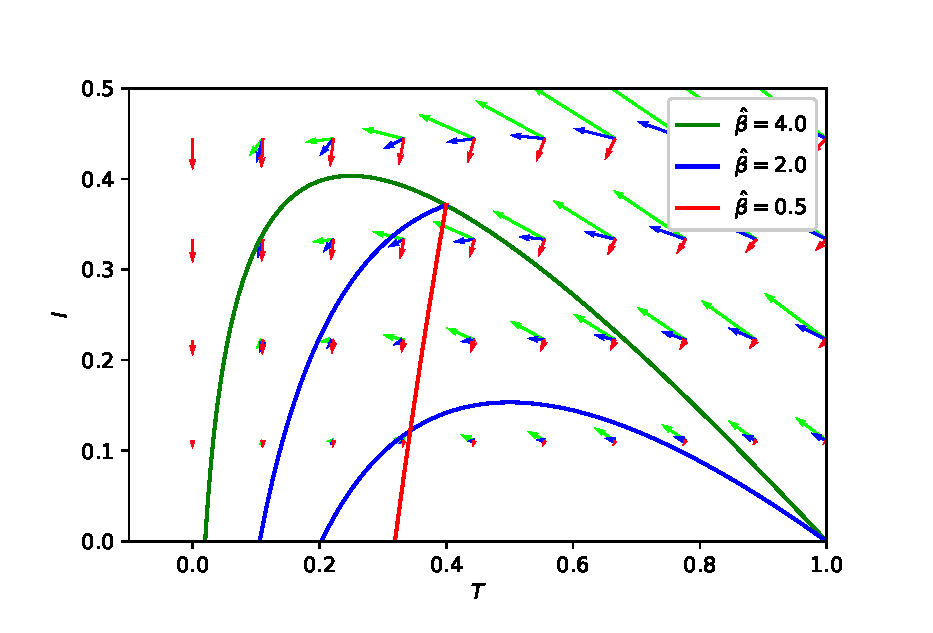
\includegraphics[width=0.9\linewidth]{figs/pp-vector-field-py}

\caption{(WIP) Phase plane: explain after the peak arrows overlap; larger beta
leads to triangle; peak at small T{*} so that change in beta after
peak has minimal effect on the VL reduction}

\end{figure}


\section{Discussion} \label{sec:discussion}
In this paper, we have conducted mathematical and simulation-based analysis of the TCL model, which meet urgent need of thorough understanding of this widely-used model. The focus is on the infection rate parameter $\beta$ which is often considered to be the parameter on which antiviral drug effect acts, especially for an antibody drug. Our simulation shows that in a typical infection, a non-monotonic relationship between the number of days above LOQ (sourjon time) and the infection rate $\beta$. This, in some sense, contradicts our expectation that drug effects speed up recovery or at least do not prolong the recovery process. Moreover, for certain intermediate $\beta$ values unrealistic sourjon time as long as 60 days is given by the model. This is likely an artifact. Although the TCL model that ignores immune responses is not intended for simulating long-term infections, the short-term slow decline of high VL for an intermediate fold change of $\beta$ from its nominal values as shown in the simulation (Fig. \ref{fig:logVL-days}) look dubious, which calls further experimental investigation to verify or dispute. Sourjon time is more suitable to simulation-based analysis. On the logarithmic scale of VL, the decline transition to be linear shortly after reaching the peak VL, which prompts us to study the asymptotic reduction rate of VL, a quantity more amenable to mathematical analysis. 

To prepare the system for mathematical analysis, we conducted nondimensionlization, a common technique which not only simplifies the paramterization but also leads to possible approximation. An assumption that viral clearance is much faster than the clearance of infected cells leads to a small parameter $\epsilon$. In the leading order, we have a planar system which significantly simplifies our analysis. Similar approximation has been applied in modeling viral dynamics \cite{Kim_2021,cangelosi2018quasi}. Since we are interested in $beta$, we employed scales that leads to a dimensionless parameter $\hat{\beta}$. With all other parameters and initial values of the target cells fixed, $\hat{\beta}$ can be directly interpreted as $\beta$. Our mathematical analysis showed that the VL reduction rate is indeed a non-monotonic function of $\hat{\beta}$. Furthermore, there is a critical value of $\hat{\beta}$ that the reduction rate is slowest. The analogical derived critical value matches well with our simulation (Left panael of Fig. \ref{fig:sojourn-time-slope}).

The timing of treating COVID-19 with an antiviral drug has been found important for its success. This is confirmed by our simulation and mathematical analysis. On the phase plane, the evolution of the infection is represented as a trajectory starting at $(1,0)$ and ends at $(T^*,0)$. The larger $\hat{\beta}$ the trajectory traces out a shape that more resembles a right triangle (think of $T$-axis as its base). The hypotenuse represent the rising stage of VL. For very large $\hat{\beta}$, the trajectory makes a sharp turn near (0,1) and then enters the declining stage of VL.  In this declining stage, $T \approx 0$ so that further reduction in $\hat{\beta}$ has minimal effects on the reduction rate of VL. It can be seen on the vector field (Fig. \ref{fig:pp-vector-field}) where the arrows overlapped for different values of $\hat{\beta}$ in the region $T\approx0$. 

Our work highlight the importance of a carefully constructed analysis to discover and understand certain intriguing parts of a mathematical model, which would otherwise be left unnoticed. TCL model we studied is widely used and standard sensitivity analysis has been done on parameter values including $\beta$ \cite{Vaidya_2021}. However, metrics like partial rand correlation failed to reveal this non-monotonic relationship.  To our knowledge, the discovery of the non-monotonic relationship between $\beta$ and disease recovery VL metric (the sourjon time and asymptotic VL reduction rate) for a TCL model is new.        

most of  Unrealistic long sourjon time  
    
nondimensionalization and beta hat

beta than standard sensitivity analysis  

standard analysis
\bibliographystyle{plain}
\bibliography{ref}

\end{document}
